\begin{frame}{Zeeman Splitting}
	\only<1->{
		\[
		\hspace*{-0.5cm}\mathcal{H} = \sum_{k}\left[h (\hat{n}_{k,\downarrow} - \hat{n}_{k,\uparrow}) + \sum_{\sigma}\epsilon_k \hat{n}_{k,\sigma}\right] 
		+V\sum_{k}	\hat{c}_{k\uparrow}^{\dagger}\hat{c}_{-k\downarrow}^{\dagger}\hat{c}_{k\uparrow}\hat{c}_{-k\downarrow}
		\]
		\vspace{0.2cm}
	}
	\begin{columns}
		\column{0.48\textwidth}
		
		\only<2->{
		\centering
		
		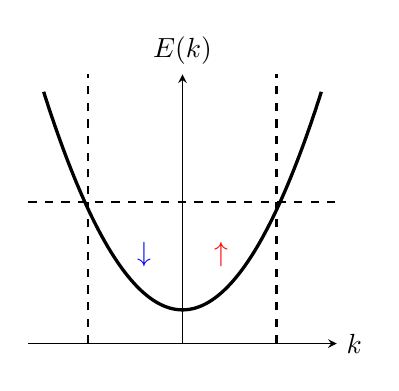
\begin{tikzpicture}
			\begin{axis}[
				width=5.5cm,
				height=5cm,
				xmin=-2, xmax=2,
				ymin=0, ymax=4,
				axis lines=middle,
				xlabel={$k$},
				ylabel={$E(k)$},
				xtick=\empty,
				ytick=\empty,
				xlabel style={at={(ticklabel* cs:1)}, anchor=west},
				ylabel style={at={(ticklabel* cs:1)}, anchor=south}
				]
				
				% Overlapping Paraboloids (Degenerate state)
				\addplot[very thick, black, domain=-1.8:1.8, samples=100] {x^2 + 0.5};
				
				% Explicit labels clear of the axis line
				\node[red, anchor=south] at (axis cs:0.5,1) {$\uparrow$};
				\node[blue, anchor=south] at (axis cs:-0.5,1) {$\downarrow$};
				
				\only<4->{
					\draw[dashed, black, thick] (-1.22,0) -- (-1.22,4);
					\draw[dashed, black, thick] (1.22,0) -- (1.22,4);
				}
				% Fermi Level
				\draw[dashed, black, thick] (-2,2.1) -- (2,2.1) node[right, black] {$E_F$};
				
			\end{axis}
		\end{tikzpicture}
	}
		\column{0.48\textwidth}
		\only<3->{
		\centering
		
		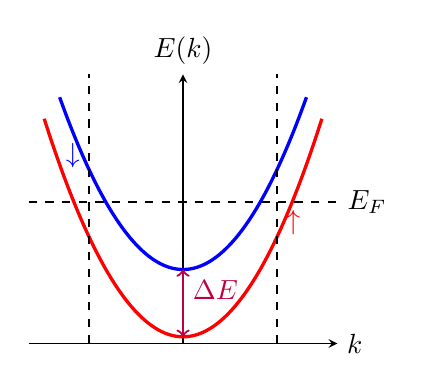
\begin{tikzpicture}
			\begin{axis}[
				width=5.5cm,
				height=5cm,
				xmin=-2, xmax=2,
				ymin=0, ymax=4,
				axis lines=middle,
				xlabel={$k$},
				ylabel={$E(k)$},
				xtick=\empty,
				ytick=\empty,
				xlabel style={at={(ticklabel* cs:1)}, anchor=west},
				ylabel style={at={(ticklabel* cs:1)}, anchor=south},
				clip=false
				]
				
				% Spin Up Band: Red Solid (Shifted Down in Energy)
				\addplot[very thick, red, domain=-1.8:1.8, samples=100] {x^2 + 0.1};
				\node[very thick, red, anchor=west] at (axis cs:1.2,1.8) {$\uparrow$};
				
				% Spin Down Band: Blue Solid (Shifted Up in Energy)
				\addplot[very thick, blue, domain=-1.6:1.6, samples=100] {x^2 + 1.1};
				\node[very thick, blue, anchor=east] at (axis cs:-1.2,2.8) {$\downarrow$};
				
				% Fermi Level
				\draw[dashed, black, thick] (-2,2.1) -- (2,2.1) node[right, black] {$E_F$};
				
								% Fermi Level
				\only<5->{
					\draw[dashed, black, thick] (-1.22,0) -- (-1.22,4);
					\draw[dashed, black, thick] (1.22,0) -- (1.22,4);
				}
				
				% Splitting Arrow (Fixed 'top, right' node position error)
				\draw[<->, thick, purple] (0,0.1) -- (0,1.1);
				\node[purple, anchor=west] at (axis cs:0,0.8) {$\Delta E$};
				
			\end{axis}
		\end{tikzpicture}
		}
		
	\end{columns}
	
\end{frame}

\begin{frame}{Spin texture and momentum transfer}
	
	\begin{columns}
		
		% =========================
		% LEFT: original picture
		% =========================
		\column{0.48\textwidth}
		\centering
		
		\only<1->{
			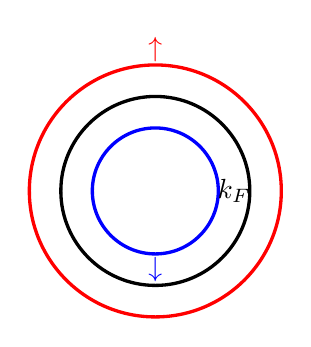
\begin{tikzpicture}
				
				% center
				\coordinate (C) at (0,0);
				
				% radii
				\def\Rbig{1.6}
				\def\Rsmall{0.8}
				\def\Rk{1.2}
				
				% big circle (spin up)
				\draw[very thick, red] (C) circle (\Rbig);
				\node[red] at (0,\Rbig+0.2) {$\uparrow$};
				
				% small circle (spin down)
				\draw[very thick, blue] (C) circle (\Rsmall);
				\node[blue] at (0,-\Rsmall-0.2) {$\downarrow$};
				
				\only<2->{
					\draw[very thick, black] (C) circle (\Rk);
					\node[black] at (\Rk-0.2,0) {$k_F$};
				}
				
			\end{tikzpicture}
		}
		
		% =========================
		% RIGHT: modified picture
		% =========================
		\column{0.48\textwidth}
		\centering
		
		\only<3->{
			\begin{tikzpicture}
				
				% parameters (changed radii)
				\def\Rbig{1.9}
				\def\Rsmall{0.6}
				
				% place centers so circles touch:
				% distance = Rbig - Rsmall (inner tangent)
				\pgfmathsetmacro{\d}{\Rbig - \Rsmall}
				
				\coordinate (Cbig) at (0,0);
				\coordinate (Csmall) at (\d,0);
				
				% big circle (spin up)
				\draw[very thick, red] (Cbig) circle (\Rbig);
				\node[red] at (0,\Rbig+0.2) {$\uparrow$};
				
				% small circle (spin down)
				\draw[very thick, blue] (Csmall) circle (\Rsmall);
				\node[blue] at (\d,-\Rsmall-0.2) {$\downarrow$};
				
				% vector Q
				\only<3>{
					\draw[->, thick, black] (Cbig) -- (Csmall)
					node[midway, above] {$\mathbf{Q}$};
				}
				\only<4->{
					\node[draw, fill=blue, fill opacity=0.2, text opacity=1,
					minimum width=0.2cm, minimum height=0.5cm] at (\Rbig,0) {};
					\node[draw, fill=blue, fill opacity=0.2, text opacity=1,
					minimum width=0.2cm, minimum height=0.5cm] at (\Rsmall+0.1,0) {};
				}
				
			\end{tikzpicture}
		}
		
	\end{columns}
	
\end{frame}